\documentclass[journal]{IEEEtran}
\usepackage[T1]{fontenc}
\usepackage{lmodern,amsmath,amssymb,graphicx,booktabs,tikz}
\usepackage[hidelinks]{hyperref}
\DeclareMathOperator{\tr}{tr}
\DeclareMathOperator{\vecop}{vec}
\DeclareMathOperator{\unvec}{unvec}
\DeclareMathOperator{\Herm}{Herm}
\DeclareMathOperator{\SINR}{SINR}
\DeclareMathOperator{\eigmax}{eig_{\max}}
\newcommand{\HH}{^{\mathsf H}}
\newcommand{\E}{\mathbb E}
\newcommand{\C}{\mathbb C}
\newcommand{\norm}[1]{\lVert #1\rVert}
\makeatletter
\newcommand{\TabRows}[1]{\@@input{#1}}
\makeatother
\providecommand{\LetterAssets}{../../results/partf-2026-11-23/assets}
\title{Fast Clutter-Aware ISAC Beamforming by Beam-Direction Pricing and Power Allocation}
\author{Muneef Mohammed}
\begin{document}
\maketitle
\setlength{\abovedisplayskip}{7pt plus 2pt minus 2pt}
\setlength{\belowdisplayskip}{7pt plus 2pt minus 2pt}
\setlength{\jot}{2pt}

\begin{abstract}
We develop block-level beamforming for wideband integrated sensing and communication with transmit-dependent clutter. At fixed receive filters, clutter-kernel linearity and Charnes--Cooper yield a power-allocation linear program (LP). A Hermitian eigenvalue oracle prices directions and bounds the covariance gap before stream recovery. On 32 matched single-thread Python draws, six and fifteen allocations gave median paired speedups of \(6.87\times\) and \(2.48\times\) over alternating semidefinite optimization, with median true sensing losses of \(0.219\) and \(0.052\) dB. A separate 96-pair study found median true losses of \(0.012\)--\(0.142\) dB at fifteen allocations across three conditions. All 288 terminal certificates covered the gaps to converged fixed-receiver references and were often loose. A two-stage learning-to-optimize (L2O) policy proposes directions from the first LP's dual prices. On unseen clutter maps, L2O shortened runtime and reduced design SCNR at matched budgets. These results support slow-timescale covariance design.
\end{abstract}

\begin{IEEEkeywords}
Integrated sensing and communication, clutter covariance, fractional programming, column generation, learning to optimize.
\end{IEEEkeywords}

\section{Introduction}
Cold-clutter covariance changes with the transmit beams, coupling target illumination and downlink interference. Liu \emph{et al.} address this coupling in a block MIMO-OFDM benchmark by alternating receive filters and transmit covariance SDPs~\cite{liu2026clutter}.

Semidefinite relaxation and rank reduction handle downlink covariance constraints~\cite{huang}. Quadratic transforms address fractional beamforming, including multiple ratios~\cite{shen}. First-order low-memory methods reduce the cost of general SDPs~\cite{yurtsever}. Here the fixed-receiver objective is one ratio of affine functions of beam powers. We apply Charnes--Cooper linearization~\cite{charnes} and use the resulting dual prices to select rank-one directions through small Hermitian eigenproblems. The same prices yield a fixed-receiver covariance bound.

\section{Block-Level Clutter Model}
A colocated system uses \(N_t\) transmit elements, \(N_r\) receive elements and \(N\) tones. The first \(K\) columns of \(W_n\) carry private streams and the other \(N_s-K\) columns carry sensing streams. Unit-covariance symbols \(s_n[\ell]\) give
\begin{align}
 x_n[\ell]&=W_n s_n[\ell],\\
 Q_n&=W_nW_n\HH,\qquad \sum_n\tr Q_n\le P .
 \label{eq:power}
\end{align}
User \(k\) sees \(h_{nk}\HH x_n[\ell]\) plus noise of variance \(\sigma_c^2\). Its SINR, with sensing included in interference, is
\begin{equation}
 \SINR_{nk}(W)=
 \frac{|h_{nk}\HH w_{nk}|^2}
 {\sum_{m\ne k}|h_{nk}\HH w_{nm}|^2+\sigma_c^2}.
 \label{eq:sinr}
\end{equation}
For a half-wavelength-spaced ULA at carrier \(f_c\), define the steering entry on \(f_n=f_c+n\Delta f\) by
\begin{equation}
 [a_M(\theta,n)]_m=\frac{\exp[-\mathrm{j}\pi m(f_n/f_c)\sin\theta]}{\sqrt M},
 \quad 0\le m<M .
\end{equation}
The steering vectors \(a_n,b_n\) use dimensions \(N_t,N_r\) and target bearing \(\theta_0\). The spatial observation is
\begin{equation}
 y_n[\ell]=\alpha_n[\ell] b_na_n\HH x_n[\ell]
             +H_{c,n}[\ell]x_n[\ell]+\omega_n[\ell].
\end{equation}
The hot clutter and sensor noise in \(\omega_n\) have fixed additive covariance \(R_{\eta,n}\). The target coefficient follows the benchmark's fixed-\(P\) convention with light speed \(c_0\), gains \(G_t,G_r\), cross section \(\sigma_{\rm rcs}\), and range \(r_0\)~\cite{liu2026clutter}
\begin{equation}
 \kappa_n=\frac{P(c_0/f_n)^2G_tG_r\sigma_{\rm rcs}}{(4\pi)^3r_0^4}.
 \label{eq:target}
\end{equation}
The expected cold-clutter response \(\mathcal C_n(Q)=\E[H_{c,n}QH_{c,n}\HH]\) is linear in the block covariance,
\begin{equation}
 \vecop(\mathcal C_n(Q))=V_n\vecop(Q),\qquad
 R_n(Q)=\mathcal C_n(Q)+R_{\eta,n}.
 \label{eq:linear}
\end{equation}
With independent scatterers of power \(\nu_{ni}\), the ideal kernel is
\begin{equation}
 V_n=\sum_i \nu_{ni}\vecop(b_{ni}b_{ni}\HH)
                         \vecop(a_{ni}a_{ni}\HH)\HH .
 \label{eq:ideal}
\end{equation}
The distributed estimate \(\widehat V_n\) uses a Choi rearrangement \(\mathcal J\) of the least-squares kernel \(V_n^{\rm LS}\). For eigenvectors \(L_n\) of \(\Herm(\mathcal J(V_n^{\rm LS}))\) and its clipped eigenvalues \(\xi_+\), the source uses
\begin{align}
 \delta_{\rm cal}&=10^{-15}\max\{1,\operatorname{mean}(\xi_+)\},\\
 \widehat V_n&=\mathcal J^{-1}\bigl(L_n
     \operatorname{diag}(\xi_++\delta_{\rm cal}\mathbf 1)L_n\HH\bigr).
\end{align}
The projection gives a PSD Choi matrix and positive covariance responses. We design with \(\widehat{\mathcal C}\) induced by \(\widehat V\) and score again with the ideal kernel to measure sensitivity to kernel error.

For any map \(\mathcal C\) and \(U=(u_n)_n\), let
\begin{equation}
 \eta(W,U;\mathcal C)=
 \frac{\sum_n \kappa_n|u_n\HH b_n|^2 a_n\HH Q_na_n}
 {\sum_n u_n\HH [\mathcal C_n(Q_n)+R_{\eta,n}]u_n}.
 \label{eq:scnr}
\end{equation}
We optimize this ratio of sums with the benchmark's distortionless normalization
\begin{subequations}\label{eq:joint}
\begin{align}
 \max_{W,U}\quad &\eta(W,U;\widehat{\mathcal C})\\
 \text{s.t.}\quad &\SINR_{nk}(W)\ge\gamma_{nk}\quad\text{for all }n,k,\\
 &\sum_n\tr Q_n\le P,\qquad u_n\HH b_n=1\quad\text{for all }n.
\end{align}
\end{subequations}

\section{Alternating Covariance Reference}
Given \(W\), the distortionless minimum-variance filter is
\begin{equation}
 u_n=\frac{R_n^{-1}b_n}{b_n\HH R_n^{-1}b_n},\qquad
 R_n=\widehat{\mathcal C}_n(Q_n)+R_{\eta,n}.
 \label{eq:mvdr}
\end{equation}
At fixed \(U\), define
\begin{equation}
\begin{aligned}
 A_n&=\kappa_n|u_n\HH b_n|^2a_na_n\HH,\quad
 d_0=\sum_n u_n\HH R_{\eta,n}u_n,\\
 C_n&=\Herm\bigl(\unvec\{\widehat V_n\HH\vecop(u_nu_n\HH)\}\bigr),
\end{aligned}
\end{equation}
where \(\Herm(M)=(M+M\HH)/2\). The adjoint replaces \(u_n\HH\widehat{\mathcal C}_n(Q_n)u_n\) by \(\tr(C_nQ_n)\), so the objective is \(F(Q)/G(Q)\) with
\begin{equation}
 F(Q)=\sum_n\tr(A_nQ_n),\quad G(Q)=d_0+\sum_n\tr(C_nQ_n).
 \label{eq:fg}
\end{equation}
Let \(X_{nk}\) denote a user covariance and \(H_{nk}=h_{nk}h_{nk}\HH\). The reference alternates~\eqref{eq:mvdr} with a sequence of Dinkelbach SDPs at fixed \(U\)~\cite{liu2026clutter,dinkelbach}. For ratio iterate \(\varrho\), the subproblem is
\begin{subequations}\label{eq:sdp}
\begin{align}
 \max_{Q,X}\quad &F(Q)-\varrho G(Q),\\
 \text{s.t.}\quad &
 (1+\gamma_{nk}^{-1})\tr(H_{nk}X_{nk}) \notag\\
 &\qquad {}\ge \tr(H_{nk}Q_n)+\sigma_c^2,\\
 &X_{nk}\succeq0,\quad Q_n\succeq0,\quad
   Q_n-\textstyle\sum_k X_{nk}\succeq0, \label{eq:sdp-psd}\\
 &\textstyle\sum_n\tr Q_n\le P . \label{eq:sdp-power}
\end{align}
\end{subequations}
The user constraints apply on all tones. The pinned CVX implementation constrains the residual in~\eqref{eq:sdp-psd} to be real symmetric, which the Python reference retains. Updating \(\varrho\gets F(Q)/G(Q)\) uses \(d_0\) even when the constant \(-\varrho d_0\) is dropped from the SDP objective. The reference uses a Gaussian start, \(30\times30\) caps, a \(10^{-3}\) relative inner tolerance and a \(0.01\) dB outer tolerance.

From a covariance solution with strictly positive desired powers, recover
\begin{equation}
 \begin{aligned}
 w_{nk}&=X_{nk}h_{nk}/\sqrt{h_{nk}\HH X_{nk}h_{nk}},\\
 S_n&=Q_n-\sum_k w_{nk}w_{nk}\HH .
 \end{aligned}
 \label{eq:recover}
\end{equation}
Cauchy--Schwarz gives \(w_{nk}w_{nk}\HH\preceq X_{nk}\), and recovery preserves the desired power. The sensing streams use the top \(N_s-K\) nonnegative modes of \(S_n\). The reference updates and stops on covariance SCNR. Reported endpoint scores use the recovered streams and each method's returned filter unless explicitly labeled as covariance scores.

\section{Direction Pricing and Power Allocation}
\subsection{Initial dictionary and power master}
Set \(g_{nk}=h_{nk}/\norm{h_{nk}}_2\) and \(G_n=[g_{n1},\ldots,g_{nK}]\). The ZF directions \(z_{nk}\) and target null direction are formed from
\begin{equation}
 Z_n=(G_n\HH)^\dagger,\qquad a_{\perp n}=(I-Z_nG_n\HH)a_n .
 \label{eq:zf}
\end{equation}
For a full-rank \(G_n\) with \(K<N_t\), the starting communication beams are
\begin{equation}
 w_{nk}^{(0)}=z_{nk}\frac{\sqrt{\gamma'_{nk}\sigma_c^2}}{\norm{h_{nk}}_2},
 \qquad \gamma'_{nk}=(1+2\cdot10^{-5})\gamma_{nk}.
\end{equation}
The start shares the remaining budget across normalized \(a_{\perp n}\) sensing vectors. We record a failed start if ZF alone exceeds the budget. The \(3K+2\) initial columns per tone comprise unit versions of \(z_{nk}\), \(a_n\), and \(a_{\perp n}+z_{nk}(g_{nk}\HH a_n)\) for each user, plus sensing versions of \(a_{\perp n}\) and \(a_n\).

Write \(v_{nj}\) and \(o_{nj}\) for an atom and its owner, with zero denoting sensing. Its power \(p_{nj}\ge0\) contributes
\begin{equation}
 Q_n=\sum_j p_{nj}v_{nj}v_{nj}\HH,\quad
 X_{nk}=\sum_{j:o_{nj}=k}p_{nj}v_{nj}v_{nj}\HH .
 \label{eq:atom}
\end{equation}
Use safe power \(P_s=(1-10^{-8})P\) and normalized powers \(x_{nj}=p_{nj}/P_s\). The coefficients for fixed \(U\) are
\begin{equation}
\begin{aligned}
 \alpha_{nj}&=(P_s/d_0)v_{nj}\HH A_nv_{nj},\\
 c_{nj}&=(P_s/d_0)v_{nj}\HH C_nv_{nj},\\
 B_{nk,j}&=\big[(1+1/\gamma'_{nk})\mathbf 1_{\{o_{nj}=k\}}-1\big]
                 |g_{nk}\HH v_{nj}|^2,\\
 d_{nk}&=\sigma_c^2/(P_s\norm{h_{nk}}_2^2).
\end{aligned}
\label{eq:coeffs}
\end{equation}
Across tones \(B\) is block diagonal. The normalized allocation satisfies \(Bx\ge d\) and \(\mathbf 1^\top x\le1\), and its SCNR is \(\alpha^\top x/(1+c^\top x)\). Nonnegative \(c\) follows from PSD clutter response. With \(s=\max_{nj}\alpha_{nj}>0\), \(\bar\alpha=\alpha/s\), \(t=1/(1+c^\top x)\), and \(y=tx\), Charnes--Cooper gives
\begin{subequations}\label{eq:lp}
\begin{align}
 \max_{y,t}\quad &\bar\alpha^\top y,\\
 \text{s.t.}\quad & By\ge dt,\quad \mathbf 1^\top y\le t,\\
 &c^\top y+t=1,\qquad y\ge0,\quad t\ge0 .
\end{align}
\end{subequations}
Feasibility implies \(t>0\). The decoded powers are \(P_s y/t\) and the attained covariance SCNR is \(s\psi\), where \(\psi\) is the optimal scaled master value.

\begin{table}[t]
 \caption{Symbols used in the optimization and audit.}
 \label{tab:symbols}
 \centering\footnotesize
 \begin{tabular}{@{}ll@{}}
 \toprule
 Symbol & Meaning\\
 \midrule
 \(\theta_0,\ \nu_{ni}\) & Target bearing and scatterer power\\
 \(\eta,\ \varrho\) & SCNR and Dinkelbach ratio iterate\\
 \(\psi,\ \mu_{nk},\ \lambda\) & Master value, SINR and power prices\\
 \(\eigmax(M),\ \epsilon\) & Largest eigenvalue and pricing excess\\
 \(\delta_{\rm cal},\ \gamma'_{nk}\) & Calibration floor and tightened SINR\\
 \(\rho\) & Correlated-channel coefficient\\
 \bottomrule
 \end{tabular}
\end{table}

\subsection{Eigenvalue oracle and fixed-receiver bound}
Let \(\mu\ge0\) and \(\lambda\ge0\) price \(dt-By\le0\) and \(\mathbf1^\top y-t\le0\). Strong duality identifies the free normalization multiplier with \(\psi\). A unit direction \(v\) at tone \(n\) and owner \(o\) has reduced cost \(v\HH M_{no}v-\lambda\), where
\begin{equation}
\begin{aligned}
 M_{n0}&=\tfrac{P_s}{d_0}(A_n/s-\psi C_n)
             -\sum_k\mu_{nk}g_{nk}g_{nk}\HH,\\
 M_{no}&=M_{n0}+(1+1/\gamma'_{no})\mu_{no}g_{no}g_{no}\HH,\quad o>0 .
\end{aligned}
\end{equation}
A principal eigenvector of \(\Herm(M_{no})\) is an exact full-sphere pricing direction~\cite{dantzig}. The standard LP schedule adds one direction for each owner with excess greater than \(10^{-7}\). Defining
\begin{align}
 \epsilon&=\max_{n,o}[\eigmax(\Herm(M_{no}))-\lambda]_+,\\
 \Delta_U&=10\log_{10}(1+\epsilon/\psi)\quad(\psi>0),
 \label{eq:bound}
\end{align}
the gap to the full fixed-receiver optimum is at most \(\Delta_U\) dB. Indeed, for any feasible full-dictionary allocation, the reduced-cost inequalities give
\begin{equation}
 \bar\alpha^\top y
 \le\psi+(\lambda-\psi-\mu^\top d)t+\epsilon\mathbf1^\top y
 \le\psi+\epsilon .
\end{equation}
The \(t\) coefficient is nonpositive by dual feasibility, and \(\mathbf1^\top y\le t\le1\). Each PSD block decomposes as a finite sum of unit rank-one directions. The restricted optimum provides the lower value \(\psi\). Appending columns at the same \(U\), scale and constraints preserves or improves this restricted optimum because zero extension preserves feasibility.

The bound applies under \(\widehat V_n\) to the tightened covariance problem at the terminal master's fixed receiver \(U\), before rank truncation. Global optimality of the joint nonconvex transceiver is outside its scope. The priced solver accepts a recovered candidate only if its nominal SINR margin is at least \(-10^{-4}\) dB, its power is within \(P(1+10^{-7})\), and its fixed-\(U\) estimated SCNR is at least \(1-10^{-10}\) times the incumbent. It refreshes \(U\) from accepted streams at the outer boundary. The terminal pass prices the final LP and adds zero columns. For \(J\) atoms the master has \(J+1\) variables, \(NK+1\) inequalities and one equality. Pricing costs \(O(N(K+1)N_t^3)\) per dense pass. Kernel application and stream recovery also contribute to runtime.

\section{Measured Results}
The benchmark uses 32 tones, \(N_t=N_r=N_s=16\), 100 W, 28 GHz and 120 kHz spacing. The numeric comparisons use the pinned matrices and preserve the original normalization in~\eqref{eq:target}. Times measure design and feasibility acceptance. Design gaps score \(\widehat V_n\) and true gaps score \(V_n\). End-to-end gaps are signed AO minus LP differences on matched streams and receivers. Bracketed intervals summarize paired bootstrap resampling unless identified as exact hit-rate intervals.

\begin{table}[t]
 \caption{Reconciliation with Fig.~12(b) for \(K=4\). True covariance SCNR is in dB. Each replay mean uses 32 draws and linear-domain averaging.}
 \label{tab:reconciliation}
 \centering\footnotesize
 \begin{tabular}{@{}lrr@{}}
 \toprule
 Data or control & \(\gamma=8\) dB & \(\gamma=12\) dB\\
 \midrule
 \TabRows{\LetterAssets/reconciliation.tex}
 \bottomrule
 \end{tabular}
\end{table}

\subsection{Reconciliation and quality tolerances}
Table~\ref{tab:reconciliation} compares true covariance scores for estimated-kernel designs. The pinned replay lies 1.58--1.60 dB below the digitized \(K=4\) curve. Stream truncation had no material effect on the 64 baseline draws at 0.001 dB resolution. The tested cap, tolerance, path-loss and fixed-coefficient power controls each shifted the mean by less than 0.05 dB. Changing only the loaded slow-time length left the two checked scores identical. The exact published Monte Carlo and calibration inputs remain unavailable. The matched timing claims use the local Python reference.

Twenty Gaussian starts on each of three draws gave median AO spreads of 0.434 dB in design SCNR and 0.280 dB in true SCNR. The prespecified \(\max(0.1\,\mathrm{dB},2\times\mathrm{median\ spread})\) rule gives tolerances of 0.867 and 0.561 dB. Under \(1\%\) relative RMS channel error, even a 1 dB explicit SINR tightening preserves all requirements for only \(38.5\%\) and \(10.6\%\) of perturbed channel realizations averaged over draws at the two thresholds. The appendix gives the perturbation model and full margin table.

\begin{table}[t]
 \caption{Single-thread Python ladder on 32 matched draws at \(K=4\) and 8 dB. Time and true SCNR are medians. B4 uses three single-SDP outer rounds. B5 uses 28 certified, physically eligible pairs.}
 \label{tab:ladder}
 \centering\footnotesize
 \setlength{\tabcolsep}{3pt}
 \begin{tabular}{@{}llrrr@{}}
 \toprule
 Arm & Configuration & Time (s) & True (dB) & Eligible\\
 \midrule
 \TabRows{\LetterAssets/ladder.tex}
 \bottomrule
 \end{tabular}
\end{table}

\subsection{Attribution and operating points}
Table~\ref{tab:ladder} uses independent seeds 16001--16032. The structured start gives a median paired speedup of \(1.44\times\) [1.35, 1.55] relative to B1, and capping that version at \(3\times2\) gives another \(1.50\times\) [1.39, 1.73]. With persistent masters on both sides, one Charnes--Cooper SDP per outer step gives \(1.12\times\) at three outer steps. Tone decomposition costs 3.361 s serially and 2.949 s with two tone workers versus 0.531 s for the serial matched joint SDP. The supplement reports iteration counts and the timed coverage.

Analytic pricing adds computation compared with random generation and improves median paired true SCNR by 1.747 dB at \(3\times2\) and 1.884 dB at \(5\times3\) with matched counts. The descriptive B1-to-B8 ratios are \(6.87\times\) [6.43, 7.29] and \(2.48\times\) [2.40, 2.59], with paired median true losses of 0.219 and 0.052 dB. These results include the combined effects of the algorithms and their numerical paths. The timed semidefinite baseline uses an audited eigencut implementation with HiGHS solving its restricted LPs. A separate native SCS cross-check concerns the first fixed-receiver SDP. The MATLAB/CVX comparative timing and parsing breakdown remain unverified.

\begin{figure}[t]
 \centering\includegraphics[width=\columnwidth]{\LetterAssets/pareto.pdf}
 \caption{Paired design gap to local AO and wall time for \(K=4\), 8 dB. Marker shapes denote outer by inner budget labels and filled markers are nondominated. CC uses one transmit SDP per outer round. The dotted line is the registered 0.867 dB tolerance.}
 \label{fig:pareto}
\end{figure}

At seeds 10001--10032, the three conditions \((K,\gamma_{\rm dB})=(4,8),(4,12),(6,8)\) give 96 matched pairs per core budget. The \(3\times2\) LP hits the design tolerance on all 96 pairs and the true tolerance on 31, 32 and 29 of 32, respectively. At \(5\times3\) the median design gaps are \(0.076,0.091,0.103\) dB and the median true gaps are \(0.012,0.064,0.142\) dB. Fig.~\ref{fig:pareto} compares all five registered budgets at \(K=4\) and 8 dB. Three endpoints in the wider sweep failed physical acceptance and used 31 paired draws. The appendix reports coverage, quartiles, intervals and empirical distributions.

\begin{figure}[t]
 \centering\includegraphics[width=\columnwidth]{\LetterAssets/certificate.pdf}
 \caption{Terminal certificate versus the observed covariance gap to a converged reference at the same fixed receiver. The dashed line denotes equality. The axes are linear near zero and logarithmic above \(10^{-4}\) dB.}
 \label{fig:certificate}
\end{figure}

\subsection{Certificate validity and priced power}
Fig.~\ref{fig:certificate} uses 288 terminal masters with three budgets. Reference continuations freeze the last master receiver, objective scale and constraints. Each converged with an audited remaining gap of at most \(10^{-4}\) dB. All nominal certificates exceeded the upper end of their reference intervals. The \(3\times2\) condition medians were 7.70--9.63 dB for the bound and 0.023--0.028 dB for the observed gap. The bound charges the largest reduced-cost excess to all scaled power, explaining its conservative behavior. Two decoded terminal allocations showed QoS shortfalls despite zero reported solver row residuals. Independent interior-point re-solves confirmed all terminal objective values within \(2.43\times10^{-9}\) dB, and the original recovered endpoints passed the physical gate.

Priced atoms received all decoded terminal LP power at \(3\times2\) and \(5\times3\). The condition medians of the share of added atoms active at termination were 19.8--19.9\% and 7.6--7.7\%, respectively, using \(10^{-8}P_s\) as the cutoff. Same-\(U\) fixed and random controls both trailed priced allocation by at least 1.99 dB in paired median design objective across the tested conditions and deployable budgets.

\begin{figure*}[t]
 \centering\includegraphics[width=\textwidth]{\LetterAssets/tracking-scaling.pdf}
 \caption{Correlated-channel time to the registered design target (left), with a fresh offline reference per frame, and array-size scaling under the common \(1\times1\) cap (right). Whiskers on the scaling curves give the interquartile range. The scaling model uses the factorized ideal map and fixed mean sensor disturbance.}
 \label{fig:tracking}
\end{figure*}

\subsection{Block timing and scope}
At 120 kHz with normal cyclic prefix, the NR slot duration is \(125\,\mu\mathrm{s}\) (3GPP TS 38.211 V18.3.0, Tables 4.2-1 and 4.3.2-1). The 36.5 ms median \(1\times1\) design time at \(K=4\) and 8 dB is about 292 slots. Correlated tracking used three updates on each of 32 chains per correlation. At \(\rho=0.99\), basis reuse cut median initial pivots from 203.5 to 4 compared with dictionary reuse alone. Cold and basis-reuse medians were 72 and 73 ms, with a paired cold-to-reuse ratio of 0.988 [0.962, 1.013]. The cold median spans about 576 NR slots. At \(\rho=0.90\) basis reuse increased runtime relative to cold starts. Fig.~\ref{fig:tracking} also shows that at 64 antennas the \(1\times1\) medians were 0.153 s for priced LP, 1.164 s for joint SDP and 6.753 s for per-tone SDP in the controlled scaling model. These timings characterize slow-timescale transceiver design.

The linearity in~\eqref{eq:linear} concerns the block transmit covariance and the averaged cold-clutter model of~\cite[Sec.~VI-A]{liu2026clutter}. In the symbol-level STAP/SLP formulation, the disturbance covariance has the form \(R_{\mathrm{cc},n}=X_n V_{\mathrm{cc},n}^{\mathrm{st}}X_n\HH\), where \(X_n\) depends on the actual waveform samples~\cite[Sec.~VI-B]{liu2026clutter}. Its quadratic dependence on those samples lies outside the block power-master derivation.

\begin{table}[t]
 \caption{Learning-to-optimize ablation on 64 held-out clutter maps. SCNR changes are paired design medians in dB with 95\% intervals. Time is the paired median ratio to analytic pricing.}
 \label{tab:learning}
 \centering\footnotesize
 \setlength{\tabcolsep}{2.5pt}
 \begin{tabular}{@{}lllr@{}}
 \toprule
 Budget & Directions & SCNR change & Time ratio\\
 \midrule
 \TabRows{\LetterAssets/learning-heldout.tex}
 \bottomrule
 \end{tabular}
\end{table}

\subsection{Learning to Optimize Beam Directions}
Figure~\ref{fig:l2o-architecture} shows how the first LP's dual prices feed the L2O policy. Its output is a unit vector in the span of the user's ZF and channel vectors, the target and the target-null direction. The reduced-cost policy maximizes \(v\HH M_{nk}v-\lambda\). The envelope policy adds a loss weighted by active scaled powers from the converged teacher. Both use first-LP features at training and deployment. The teacher supplied 5,000 labels, and finite differences validated both gradients.

\begin{figure}[t]
 \centering
 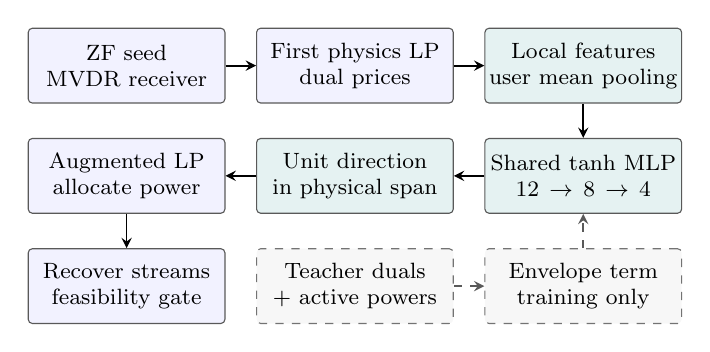
\begin{tikzpicture}[
    x=1mm,y=1mm,
    font=\footnotesize,
    block/.style={draw=black!65,rounded corners=1.5pt,align=center,
        text width=24mm,minimum height=9.5mm,inner sep=1.4pt,fill=white},
    physics/.style={block,fill=blue!5},
    learned/.style={block,fill=teal!10},
    training/.style={block,draw=black!55,dashed,fill=black!3},
    flow/.style={->,>=stealth,line width=.65pt},
    supervise/.style={flow,dashed,draw=black!65}
]
\node[physics] (seed) at (0,0) {ZF seed\\MVDR receiver};
\node[physics] (first) at (29,0) {First physics LP\\dual prices};
\node[learned] (features) at (58,0) {Local features\\user mean pooling};
\node[learned] (net) at (58,-14) {Shared tanh MLP\\\(12\to8\to4\)};
\node[learned] (beam) at (29,-14) {Unit direction\\in physical span};
\node[physics] (next) at (0,-14) {Augmented LP\\allocate power};
\node[physics] (recover) at (0,-28) {Recover streams\\feasibility gate};
\node[training] (teacher) at (29,-28) {Teacher duals\\+ active powers};
\node[training] (loss) at (58,-28) {Envelope term\\training only};
\draw[flow] (seed) -- (first);
\draw[flow] (first) -- (features);
\draw[flow] (features) -- (net);
\draw[flow] (net) -- (beam);
\draw[flow] (beam) -- (next);
\draw[flow] (next) -- (recover);
\draw[supervise] (teacher) -- (loss);
\draw[supervise] (loss) -- (net);
\end{tikzpicture}

 \caption{Two-stage learning to optimize. Solid arrows show deployment. The dashed path contributes only to envelope training. The augmented LP allocates power over the expanded dictionary.}
 \label{fig:l2o-architecture}
\end{figure}

\smallskip\noindent\begin{minipage}{\columnwidth}\footnotesize
\textbf{Algorithm 1. Fixed-budget design with L2O}
\begin{enumerate}
 \setlength{\itemsep}{0pt}\setlength{\parsep}{0pt}
 \item Initialize feasible ZF streams, dictionary and MVDR filters.
 \item At each inner step solve the power LP, recover streams, and accept the candidate only if it passes the physical and fixed-receiver SCNR gates.
 \item At the first nonterminal pass append one learned direction per user and one analytic sensing direction per tone. At later nonterminal passes append one analytic direction for each owner and tone.
 \item At the terminal pass compute the eigenvalue bound and append no atoms. Refresh MVDR from the accepted streams at every outer boundary and return the final accepted streams and filters.
\end{enumerate}
\end{minipage}\par\smallskip

Table~\ref{tab:learning} uses 64 unseen maps. The supplement includes 64 original-map draws. All 1,920 endpoints passed the physical checks. At \(1\times1\) the shared master returns identical scores. On unseen maps at \(2\times1\), both learned arms reduce median paired design time by about 10--12\%, with design SCNR losses of 0.209--0.255 dB. At \(3\times2\) the losses shrink to about 0.012 dB. The matched random baseline has a comparable median gap at six solves. The envelope policy's first-pass user proposals never cross the positive-power threshold in either cohort. Its paired median SCNR changes from reduced cost alone are below 0.000061 dB in magnitude. The archived SPSA arm awaits its original checkpoint.

\section{Reproducibility and Conclusion}
The reproducibility package includes code, locks, raw records and regeneration commands on the \href{https://github.com/muneefo/clutter_aware_beamforming-for-ISAC/tree/letters-revision}{project revision branch}. The tutorial input revision is \texttt{0f864c4}. The Python measurements use CPython 3.12.14, SciPy 1.17.0 and HiGHS 1.8.0 on an Intel Xeon Platinum 8573C. The serial ladder uses one pinned CPU and one BLAS and solver thread. The parallel tone condition uses two one-thread workers. The appendix and manifests give all seed bands and environment details.

Clutter-kernel linearity supports a power LP with analytic direction pricing and a fixed-receiver covariance certificate. The matched Python ladder shows speedups over the joint AO--SDP reference, and the expanded cohort reports small median gaps at fifteen allocations under both scoring kernels. Basis reuse reduces initial simplex work on highly correlated channels, with no demonstrated wall-time advantage over a fresh start there. The L2O direction policies yield a speed--SCNR trade-off at the measured budgets. The absolute times support slow-timescale block updates.

\bibliographystyle{IEEEtran}
\bibliography{letters}
\end{document}
